\scanpage{38}
\deleted{Dans l'inégalité (\unsure{31}), faisons \illegible{1} $p$ vers $+\infty$ et $q$ vers $0$, alors $s=\dfrac{1}{\frac1p+\frac1q}$ \deleted{\unsure{tend}} \unsure{tend} vers $0$, et \deleted{\illegible{2}} on \unsure{obtient} à la limite \illegible{1} $\unsure{\rho_i(u)}$.}

\deleted{\uline{\unsure{Rappels et notations}}} \uline{Préliminaires}

L'espace $\overline E$. Si $E$ est un Hilbert, $\overline E$ est un Hilbert, et
\[
(*)\qquad \boxed{E'=\overline E}.
\]
Propriété d'approximation : corollaire : op. \unsure{cpts} sont limites d'op. de rang fini. Bicontinuité de $E\widehat\otimes F\longrightarrow L(\overline E,F)$.

Adjoint de $u:E\longrightarrow F$ est $u^*:F\longrightarrow E$, propriétés formelles, \deleted{dont la propriété spéciale}
\[
(**)\qquad \boxed{\|u^*u\|=\|u\|^2}.
\]
Décomposition spectrale d'un hermitien \inserted{compact} : $u=\sum\unsure{\rho_i|\lambda_i}\overline e_i\otimes e_i$, où $\lambda_i\longrightarrow0$, $\lambda_i=\overline\lambda_i$. \illegible{1} $u\geq0\Longleftrightarrow\lambda_i\geq0$ pour tout \unsure{$i$}.

\margin{\uuline{\unsure{Corollaire}}}
Racine carrée d'un \illegible{1} hermitien positif compact.

Décomposition canonique \illegible{1} \unsure{n'importe quel} $u:E\longrightarrow F$.
On \deleted{\unsure{considère}} \inserted{introduit} $\sqrt{u^*u}\unsure{{}={}|{}\equiv{}}\unsure{|u|}$ op. positif dans $E$, et on a
\[
\||u|.x\|=\unsure{\|ux\|}\qquad\unsure{\forall x},
\]
d'où $ux=U|u|x$, où $U:\inserted{E\longrightarrow F}$ \unsure{défini} et isométrique sur $|u|(E)$, et qu'on donc peut prolonger en un op. de norme $\leq1$ de $E$ dans $F$, isométrique sur \deleted{\unsure{\illegible{1}} $u(E)$} l'adhérence de \deleted{$u(E)$} $|u|(E)\subset E$. Et de même
\[
|u|=Vu,
\]
où $V:F\longrightarrow E$ est de norme $\leq1$, isométrique sur l'adhérence de $u(E)\subset F$. \uline{D'où}
\[
(***)\qquad\boxed{u=U|u|\qquad |u|=Vu}\qquad(\|U\|\leq1,\ \|V\|\leq1).
\]
\inserted{En particulier $\boxed{\|u\|=\||u|\|}$, ce qui résulte aussi de $\|u^*u\|=\|u\|^2$.}

\margin{\figure{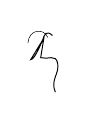
\begin{tikzpicture}[x=0.6cm,y=0.6cm]
\draw[line width=0.18pt] (0.08,1.08) .. controls (0.10,1.38) and (0.42,1.40) .. (0.50,1.20);
\draw[line width=0.35pt] (0.60,1.24) .. controls (0.48,1.35) and (0.43,1.28) .. (0.39,1.14) -- (0.14,0.73) .. controls (0.23,0.72) and (0.40,1.18) .. (0.42,1.20) -- (0.35,0.77) .. controls (0.50,0.72) and (0.67,0.86) .. (0.71,0.65) .. controls (0.75,0.42) and (0.55,0.31) .. (0.66,0.04);
\end{tikzpicture}}}

Décomposition spectrale \deleted{\unsure{de}} $|u|=\sum\ell_i\overline e_i\otimes e_i$, (les $\ell_i\geq0$)
on aura
\[
(****)\qquad\boxed{u:\sum\ell_i\deleted{\unsure{f_i}}\overline e_i\otimes f_i},
\]
où $f_i=Ue_i$, les $f_i$ forment un système orthonormal. \deleted{\illegible{3}}
\deleted{\unsure{On a de plus} $u^*=\sum\ell_i\overline f_i\otimes\unsure{e_i}$}.
Réciproquement, via une telle décomposition, on tire $|u|=\sum\ell_i\overline e_i\otimes e_i$, donc les $\ell_i$ sont les valeurs propres de $|u|$, et les $e_i$ les vecteurs propres correspondants, \unsure{on tire|les $f_i$} de ****
\[
u^*=\sum\ell_i\overline f_i\otimes e_i,
\]
donc \uuline{$|u^*|$ a les mêmes valeurs propres que $|u|$}. \unsure{\illegible{1}}
\mspage{39}
